\chapter{Experimentos}\label{cap:experimentos}

Neste capítulo são apresentados o protocolo experimental e resultados de todas as etapas e experimentos deste trabalho. Os resultados das seções sobre a base de dados (\ref{sec:expBase}) e segmentação de imagens (\ref{sec:expSegmentacao}) são apresentados de forma cronológica, enquanto os resultados da seção de classificação (\ref{sec:expClassificacao}) e suas subseções são apresentados de forma não-cronológica, privilegiando a ordem das abordagens conforme descritas na metodologia (capítulo \ref{cap:metodologia}).

\section{Base de dados}\label{sec:expBase}

A base de dados (imagens) utilizada advém do projeto GEOMA \cite{geoma}, financiado pelo Instituto Nacional de Pesquisas Espaciais (INPE). Trata-se de imagens coloridas, codificadas em JPEG e com 640 pixels de largura por 480 pixels de altura. A base é composta por fotografias ortogonais ao relevo (como pode ser visto na figura \ref{fig:amostra}), de altitudes variadas e tiradas a partir de aeronaves tripuladas, durante o trajeto entre diversas cidades da região amazônica.

No momento do início dos experimentos deste trabalho, estas imagens tiradas de aviões tripulados eram as únicas da região da Amazônia legal disponíveis publicamente. Podemos considerá-las válidas por terem sido tiradas em altitude de voo compatível com as missões de VANTs de vigilância, entre 900 e 1.100 metros do solo. Como este trabalho tem como objetivo utilizar apenas câmeras de espectro visível, são dispensáveis comparações de sensores com VANTs que eventualmente possuam sonar, câmeras infravermelho ou outros tipos de sensores.

\begin{figure}[h]
  \centering
  \begin{subfigure}[b]{0.3\textwidth}
    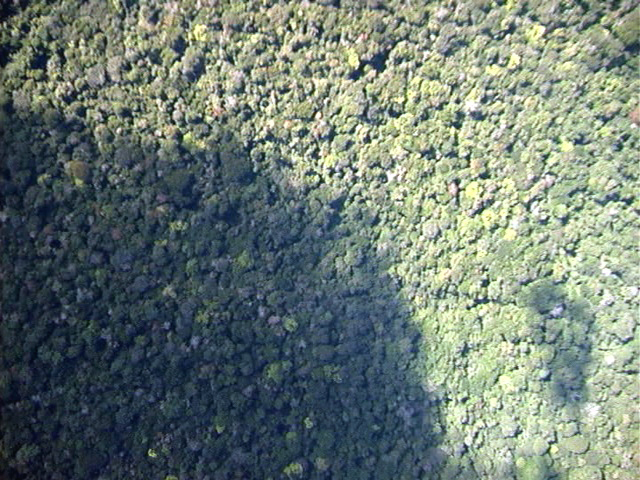
\includegraphics[width=\textwidth]{imgs/amostra1}
  \end{subfigure}%
  ~
  \begin{subfigure}[b]{0.3\textwidth}
    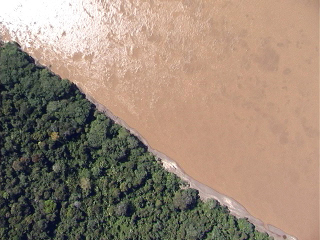
\includegraphics[width=\textwidth]{imgs/amostra2}
  \end{subfigure}%
  ~
  \begin{subfigure}[b]{0.3\textwidth}
    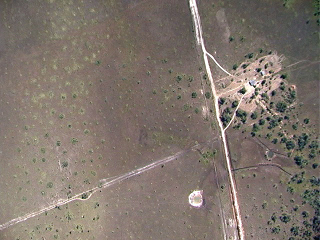
\includegraphics[width=\textwidth]{imgs/amostra3}
  \end{subfigure}%
  \caption{Amostras da base de dados}
  \label{fig:amostra}
\end{figure}

A base possui um total de 3.044 imagens, com dimensão total de 1,02 Gigabytes de dados. Todas as imagens foram utilizadas no presente trabalho sem tratamento ou manipulação prévios.

Para criar uma referência (\textit{ground-truth}) para a segmentação das imagens da base de dados, uma ferramenta computacional executável em navegadores web foi construída (figura \ref{fig:manualseg}). A saída deste aplicativo é uma coleção, para cada imagem, de informações sobre bordas das regiões da imagem. Estas informações serviram de referência para avaliar o desempenho dos algoritmos de segmentação testados neste trabalho.

\begin{figure}[h]
  \centering
  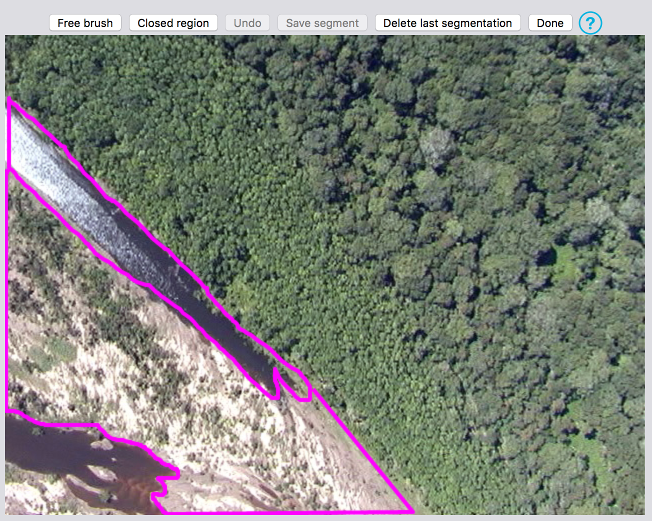
\includegraphics[width=0.7\textwidth]{imgs/manualseg}
  \caption{Ferramenta para segmentação manual das imagens}
  \label{fig:manualseg}
\end{figure}

Um dos objetivos específicos deste trabalho é a criação e disponibilização de uma base de imagens aéreas da floresta amazônica, com seus segmentos definidos, devidamente rotulados e elementos antrópicos assinalados. Esta base de imagens está publicamente disponível\footnote{http://github.com/luizcavalcanti/geoma-database}, e pode ser utilizada em diversos trabalhos futuros com temas relacionados.

\section{Segmentação}\label{sec:expSegmentacao}

Um experimento de comparação entre diversos algoritmos de segmentação de imagens foi planejado. Cada imagem da base de dados foi segmentada por seres humanos, segmentações estas que constituíram a base de referência para o experimento. Cada imagem tem sua segmentação de referência consolidada a partir da segmentação manual de pelo menos 5 indivíduos.

\subsection{Protocolo experimental}

Para criação da segmentação manual de referência (\textit{ground-truth}), 31 voluntários, todos alunos de pós-graduação em informática ou áreas relacionadas, foram convidados a realizar a segmentação manual das imagens da base de dados, através de uma ferramenta\footnote{http://amazonsegmentation.ddns.net/} criada com esta finalidade.

A ferramenta de software web criada consiste de uma interface gráfica onde o usuário pode desenhar sobre uma imagem a ser segmentada. A ideia é que nesta imagem sejam circunscritas as bordas das regiões definidas pelo usuário, de acordo com instruções fornecidas pela ferramenta e que foram lidas obrigatoriamente por cada voluntário antes do início do experimento.

Em linhas gerais, as instruções orientaram os participantes do experimento a segmentar as imagens de acordo com a cobertura ou tipo de terreno, formação geológica ou vegetação, utilizando os critérios e granularidade que lhes pareçam mais adequados:

\begin{citacao}[english]
Your mission is to manually segment the given images as accurately as possible, according to your own judgment. The criteria here is terrain coverage. So, we would like to separate different vegetations, geological formations and human-made objects. \cite{amazonsegmentation}
\end{citacao}

Em tradução livre:

\begin{citacao}
Sua missão é segmentar manualmente as imagens disponibilizadas o mais precisamente possível, de acordo com o seu julgamento. O critério aplicado é a cobertura de terreno. Portanto, nós gostaríamos de separar diferentes vegetações, formações geológicas e objetos feitos por seres humanos. \cite{amazonsegmentation}
\end{citacao}

O conteúdo integral das instruções pode ser encontrado no apêndice \ref{apendice:instrucoesManualSeg}.

\subsection{Resultados}

Antes de analisar o desempenho de cada algoritmo de segmentação investigado neste trabalho em relação à segmentação manual, foi preciso aferir a validade da própria segmentação manual, visto que ela foi realizada por diferentes participantes com diferentes interpretações das instruções fornecidas. Segundo \citeonline{martin:2001}, uma forma de validar a consistência das segmentações manuais é medir a consistência entre segmentações de uma mesma imagem feita por diferentes pessoas.

Utilizando as métricas de erro de consistência local (LCE) e global (GCE) para medir a similaridade das segmentações manuais, os resultados confirmam a consisência da segmentação manual feira pelos participantes do experimento. Conforme pode ser visto nas figuras \ref{fig:manual_gce} e \ref{fig:manual_lce}, os coeficientes de erro global e local, respectivamente, ficam abaixo dos 20\% e 10\% para todos os casos.

\begin{figure}[h]
  \centering
  \begin{subfigure}[b]{0.5\textwidth}
    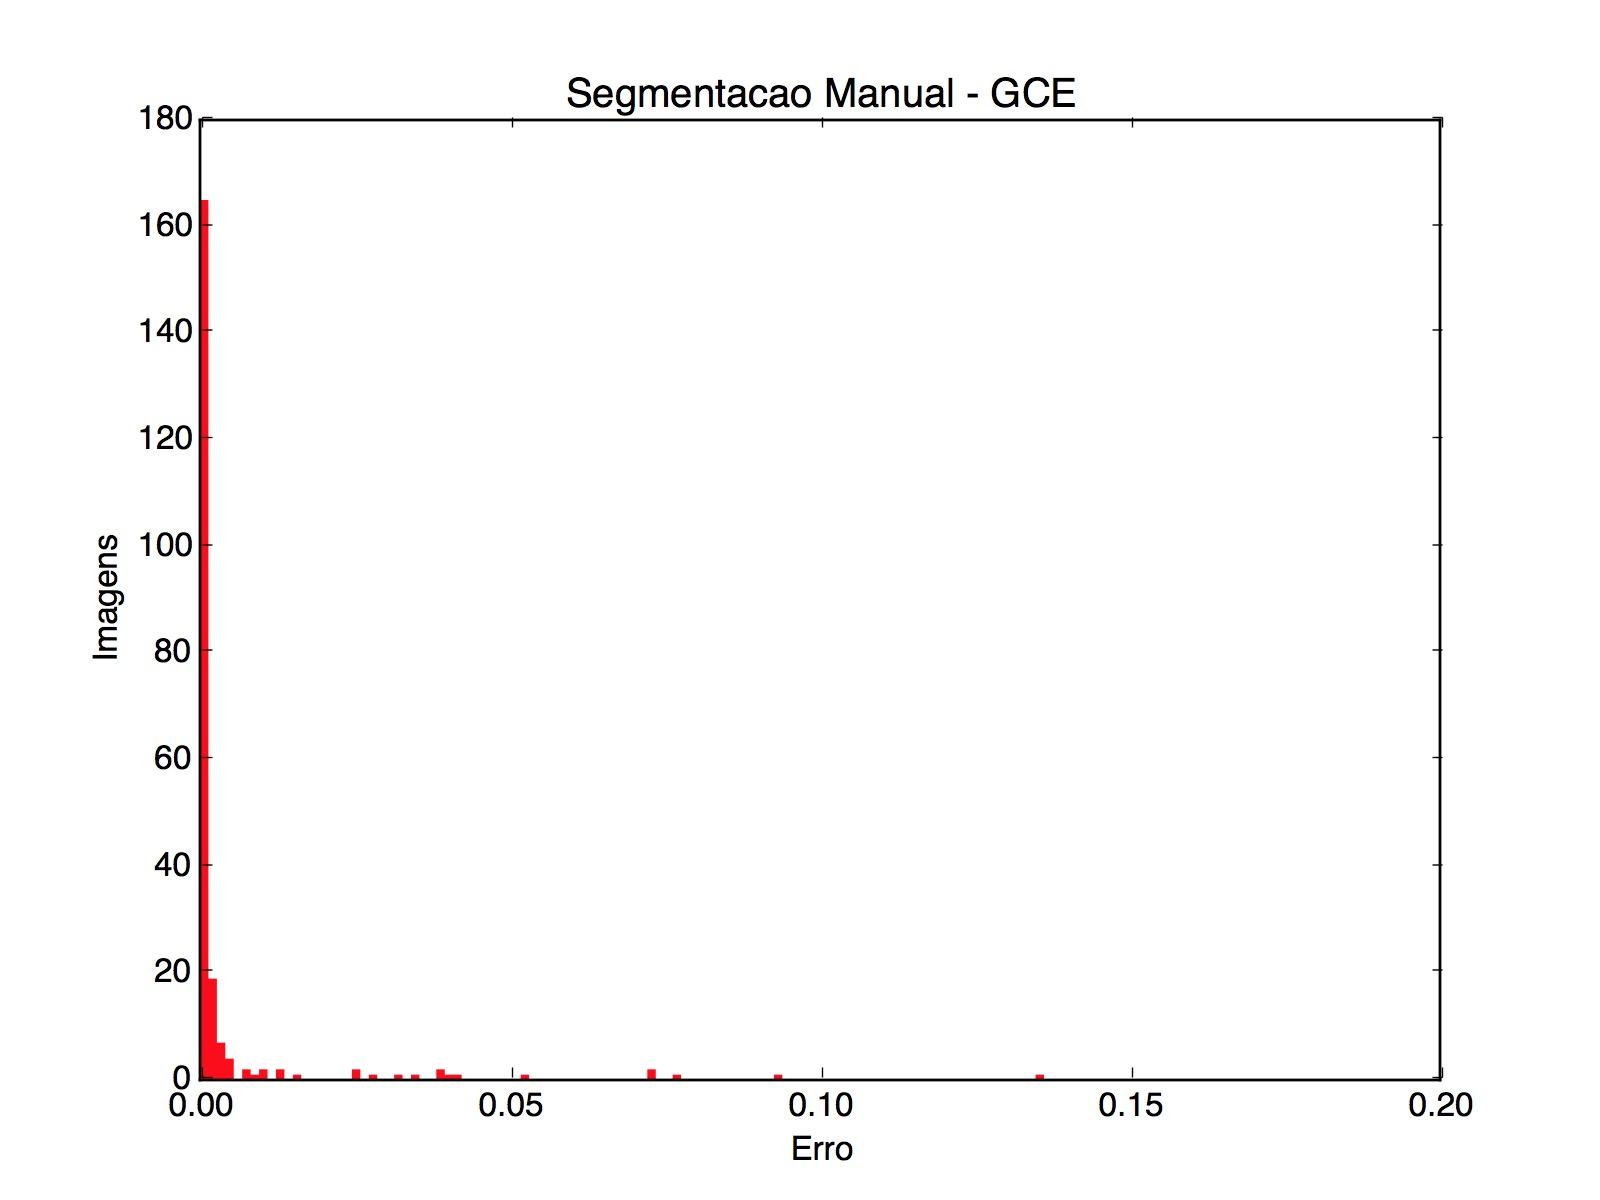
\includegraphics[width=\textwidth]{imgs/manual_gce}
  \end{subfigure}%
  ~
  \begin{subfigure}[b]{0.5\textwidth}
    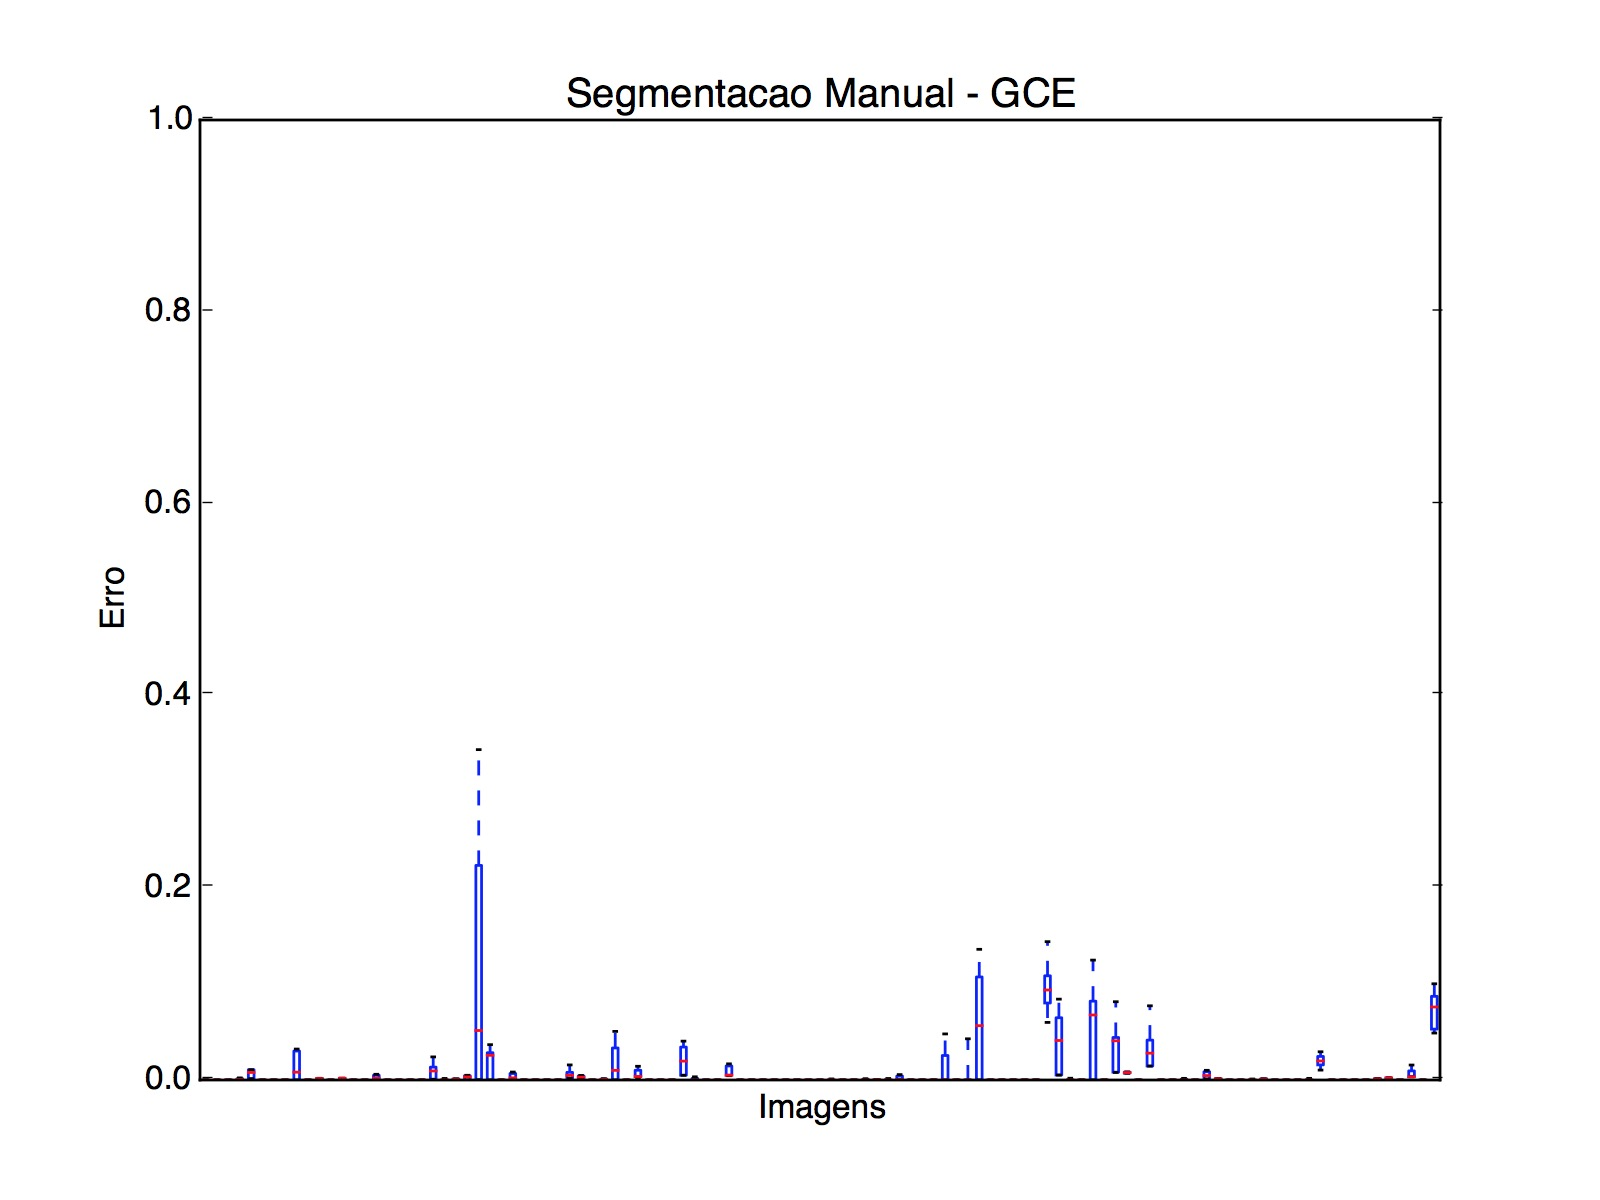
\includegraphics[width=\textwidth]{imgs/manual_dist_gce}
  \end{subfigure}%
  \caption{Coeficiente de erro global das diferentes segmentações de mesma imagem}
  \label{fig:manual_gce}
\end{figure}

\begin{figure}[h]
  \centering
  \begin{subfigure}[b]{0.5\textwidth}
    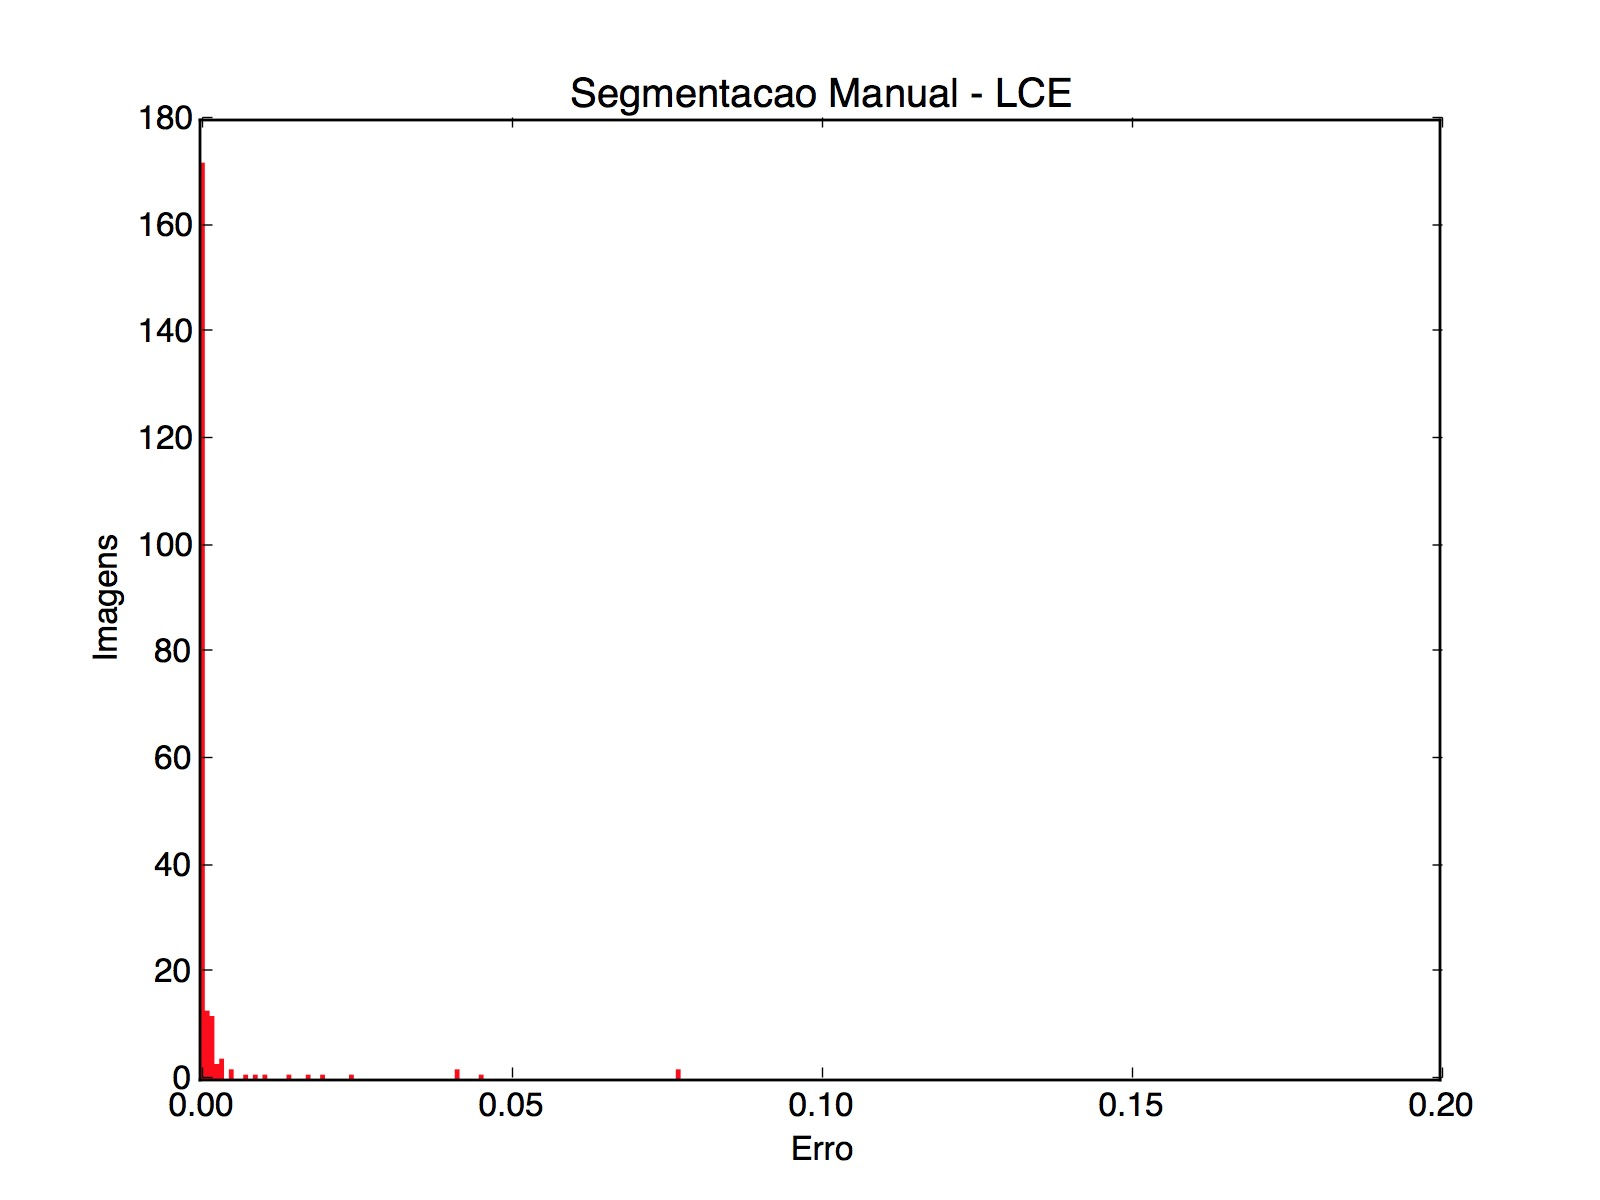
\includegraphics[width=\textwidth]{imgs/manual_lce}
  \end{subfigure}%
  ~
  \begin{subfigure}[b]{0.5\textwidth}
    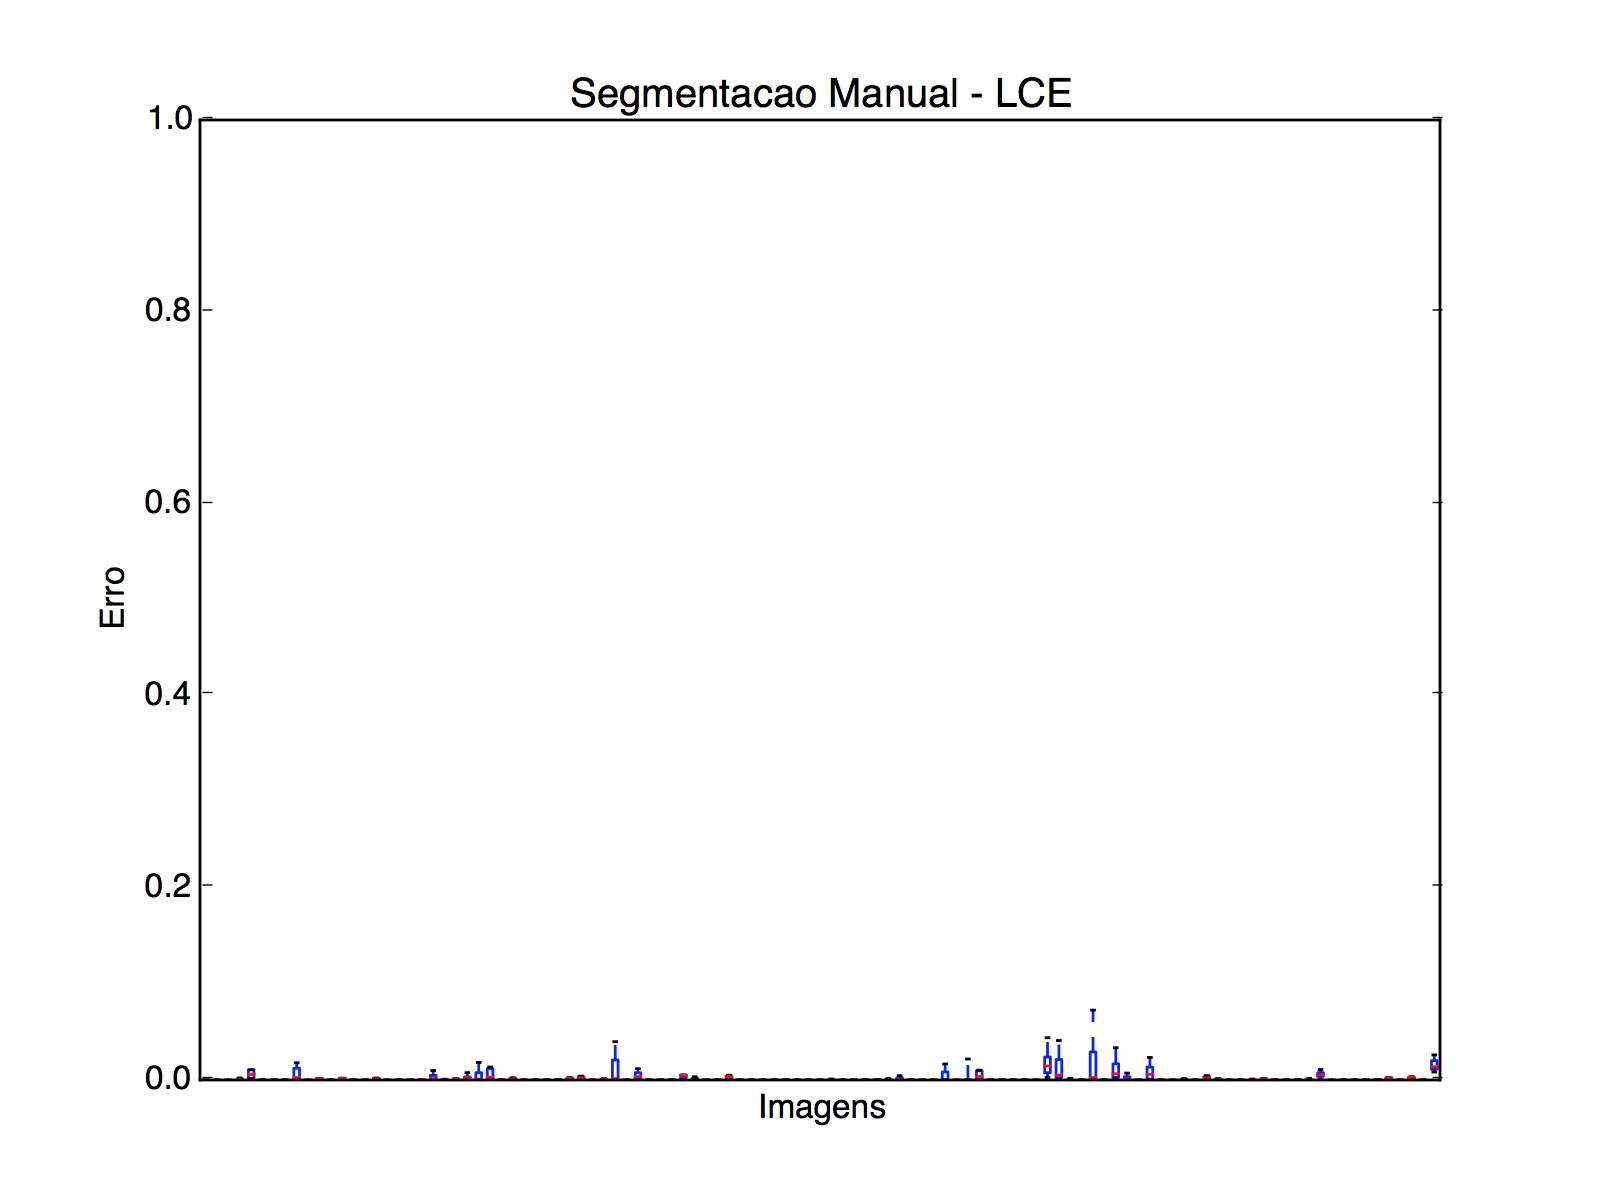
\includegraphics[width=\textwidth]{imgs/manual_dist_lce}
  \end{subfigure}%
  \caption{Coeficiente de erro local das diferentes segmentações de mesma imagem}
  \label{fig:manual_lce}
\end{figure}

Para determinar qual dos algoritmos de segmentação levantados na pesquisa bibliográfica teria melhor desempenho na base de dados utilizada neste trabalho, todos foram implementados ou adaptados. Os algoritmos foram testados em todas as imagens da base de dados do trabalho que possuíam segmentação manual por pelo menos 5 voluntários, um total de 203 imagens, utilizando as mesmas medidas de erro global (GCE) e erro local (LCE) apresentados no trabalho de \citeonline{martin:2001} e na validação da base de segmentação manual construída para este trabalho.

Os resultados do experimento são apresentados na tabela \ref{tab:experimentoSegmentacao}, com o melhor resultado para cada critério destacado em coloração cinza.

\begin{table}[h]
\centering
\begin{tabulary}{\linewidth}{|L|R|R|R|}
\hline
\textbf{Algoritmo} & \textbf{GCE médio} & \textbf{LCE médio} & \textbf{Tempo (s)} \\ \hline
Manual      & 0.01822          & 0.00537         & - \\ \hline
FSEG        & 0.03063          & 0.00273         & 13,91 \\ \hline
gPb-owt-ucm & 0.00655          & 0.00297         & 237,32 \\ \hline
JSEG        & 0.02990          & 0.00486         & 14,82 \\ \hline
Mean-shift  & 0.02237          & 0.00271         & 6,39 \\ \hline
MSEG        & 0.01005          & 0.00072         & \cellcolor{gray!25} 0,33 \\ \hline
SRM         & \cellcolor{gray!25} 0.00622 & \cellcolor{gray!25} 0.00066 & 4,66 \\ \hline
\end{tabulary}
\caption{Comparação de métodos de segmentação em parte da base de imagens deste trabalho, em ordem alfabética}
\label{tab:experimentoSegmentacao}
\end{table}

O método SRM conseguiu uma média de erros global e local substancialmente menor que os demais algoritmos e foi considerado o método com melhor desempenho do experimento na base de imagens deste trabalho, embora o tempo de segmentação deste algoritmo seja uma ordem de magnitude maior que o algoritmo MSEG, que obteve o melhor tempo de execução. A imagem \ref{fig:comparacaoSegmentacao} mostra a saída de alguns dos métodos testados, para fins de comparação visual.

\begin{figure}[htb]
	\centering
	\begin{minipage}[l]{0.32\linewidth}
		\begin{subfigure}[b]{\linewidth}
			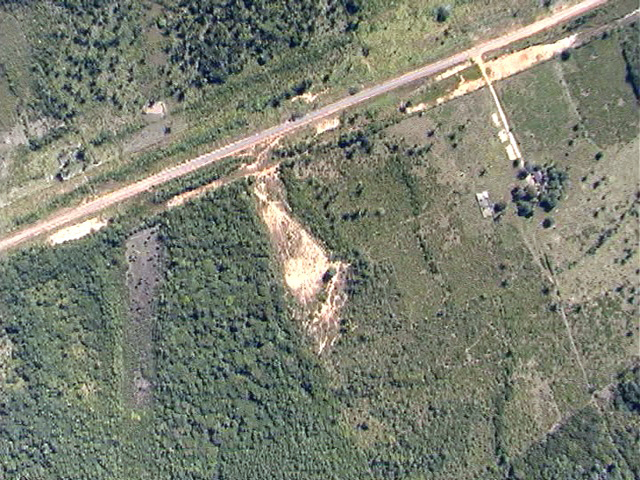
\includegraphics[width=\linewidth]{imgs/seg_original}
			\caption{Imagem original}
		\end{subfigure}%
	\end{minipage}
	\begin{minipage}[r]{\linewidth}
		\begin{subfigure}{.32\linewidth}
			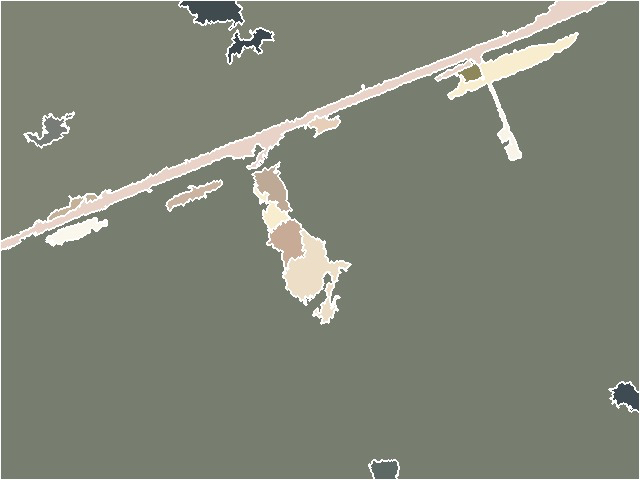
\includegraphics[width=\linewidth]{imgs/seg_meanshift}
			\caption{Mean-shift}
		\end{subfigure}
		\begin{subfigure}{.32\linewidth}
			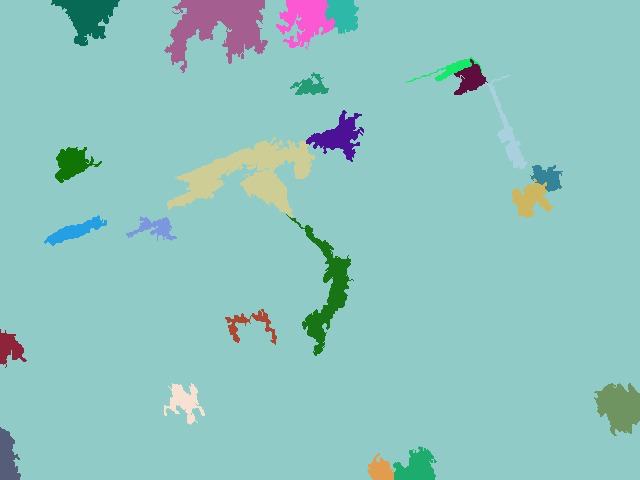
\includegraphics[width=\linewidth]{imgs/seg_mseg}
			\caption{MSEG}
		\end{subfigure}
		\begin{subfigure}{.32\linewidth}
			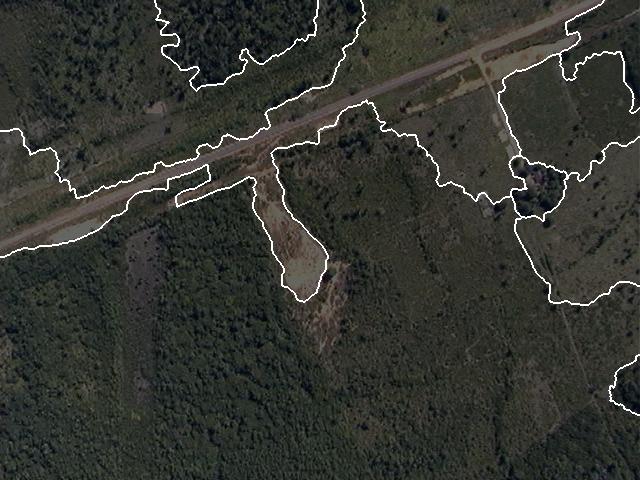
\includegraphics[width=\linewidth]{imgs/seg_jseg}
			\caption{JSEG}
		\end{subfigure}
	\end{minipage}
	\begin{minipage}[r]{\linewidth}
		\begin{subfigure}{.32\linewidth}
			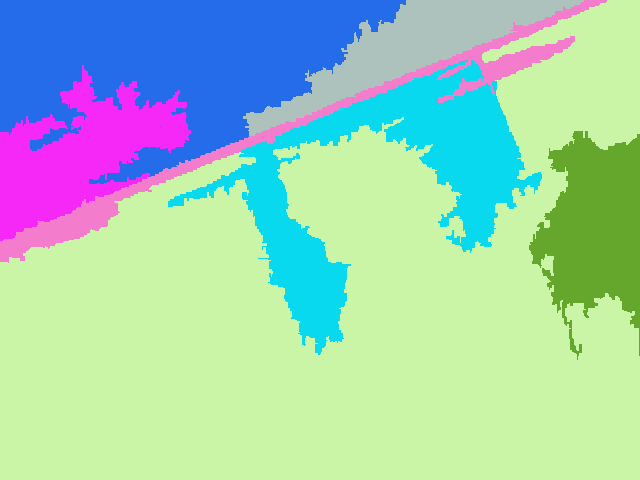
\includegraphics[width=\linewidth]{imgs/seg_srm}
			\caption{SRM}
		\end{subfigure}
		\begin{subfigure}{.32\linewidth}
			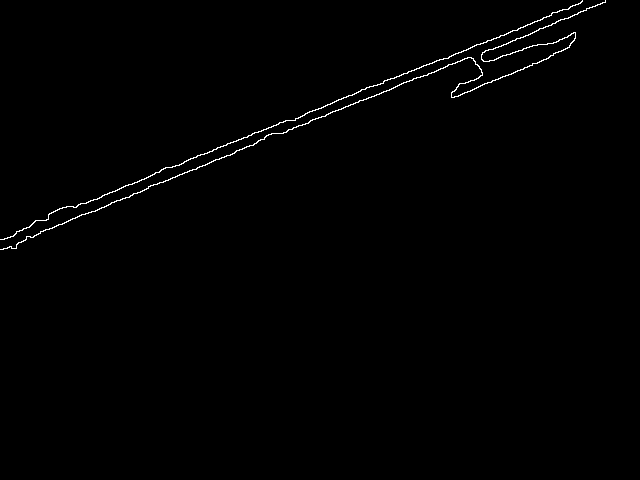
\includegraphics[width=\linewidth]{imgs/seg_gpb}
			\caption{gPb-owt-ucm}
		\end{subfigure}
		\begin{subfigure}{.32\linewidth}
			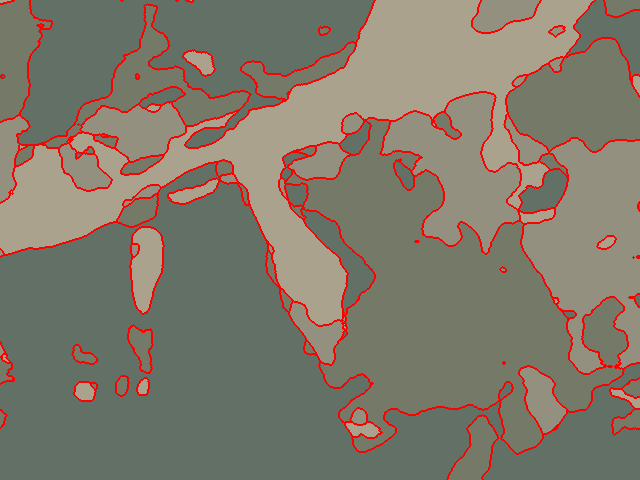
\includegraphics[width=\linewidth]{imgs/seg_fseg}
			\caption{FSEG}
		\end{subfigure}%
	\end{minipage}
	\caption{Comparação visual de métodos de segmentação}
	\label{fig:comparacaoSegmentacao}
\end{figure}


Adicionalmente, experimentos foram realizados com técnicas de classificação. O objetivo era saber se poderíamos utilizar apenas uma etapa para realizar segmentação e o primeiro nível de classificação. Todos os algoritmos obtiveram precisão inferior ao que foi conseguido na etapa de segmentação isoladamente. Os resultados foram publicados no \textit{$10^{th}$ International Conference on Computer Vision Theory and Applications} e o artigo de \citeonline{cavalcanti:2015} completo pode ser visto no apêndice \ref{cap:visapp2015}.

Para fins de comparação, os resultados deste segundo experimento são apresentados na tabela \ref{tab:experimentoArtigo}. O tempo de execução da classificação para cada imagem no artigo publicado ignora o tempo de extração de características da imagem. Para uma comparação correta com os métodos de segmentação experimentados anteriormente, esse tempo gasto em extração de características foi acrescido na tabela desta seção.

\begin{table}[h]
\centering
\begin{tabulary}{\linewidth}{|L|R|R|}
\hline
\textbf{Algoritmo} & \textbf{Acurácia} & \textbf{Tempo/imagem} \\ \hline
Random forest  & \cellcolor{gray!25} 96,0\% & 12,72 s \\ \hline
KNN            & 92,6\%                     & 22,89 s \\ \hline
Naive Bayes    & 92,8\%                     & \cellcolor{gray!25} 8,36 s \\ \hline
Decision tree  & 82,2\%                     & 14,49 s \\ \hline
\end{tabulary}
\caption{Comparação de métodos de classificação para segmentação das imagens em uma única etapa, ordenados por acurácia}
\label{tab:experimentoArtigo}
\end{table}

Os segmentos encontrados pelo algoritmo SRM, escolhido nesta etapa, serviram de entrada para a próxima etapa da solução, responsável pela classificações destes mesmos segmentos.

\section{Classificação}\label{sec:expClassificacao}

A segunda etapa da solução consiste em classificar os segmentos de imagens produzidos na etapa de segmentação. Uma conjunto de experimentos foi realizado com base nas quatro abordagens para classificação supervisionada, descritas no capítulo \ref{cap:metodologia}:

\begin{itemize}
	\item Classificadores multi-classe
	\item Classificadores binários
	\item Classificadores unários
	\item Conjunto de classificadores unários
\end{itemize}

\subsection{Protocolo experimental}

Primeiramente, todas as imagens foram segmentadas utilizando o algoritmo SRM, por conta de seu melhor desempenho no experimento de segmentação anterior. Cada um dos 10.057 segmentos produzidos nesta segmentação foi devidamente classificado manualmente, e suas características foram extraídas. Cada segmento foi classificado como uma das possíveis classes para o problema: floresta, vegetação rasteira, água, terra ou elemento antrópico.

Cerca de 70 segmentos não puderam ser classificados, pois continham mais de um tipo de terreno dentro de seus limites, tornando a rotulação dúbia. É importante destacar que nenhum destes segmentos continha elementos antrópicos, portanto, foram descartados da base utilizada no treinamento e validação dos modelos de aprendizado.

Todos os elementos antrópicos encontrados foram validados pela Dra. Solange Costa, especialista do Centro Gestor e Operacional do Sistema de Proteção da Amazônia (CENSIPAM), órgão governamental federal responsável pelo patrulhamento e sensoriamento remoto da Amazônia legal brasileira.

Em seguida, uma análise da base de segmentos rotulada foi feita, observando a estrutura e a distribuição dos dados ao longo de toda a base, levando em consideração como os tipos de dados utilizados e sua representação podem influenciar os resultados dos algoritmos de aprendizado utilizados no experimento.

Após a rotulação de todas as amostras utilizadas no experimento, a distribuição das classes do problema em toda a base foi medida e pode ser vista na tabela \ref{tab:experimentoRegioesDistribuicao}.

\begin{table}[h]
\centering
\begin{tabulary}{\linewidth}{|L|R|R|}
\hline
\textbf{Classe} & \textbf{Amostras} & \textbf{Percentual} \\ \hline
Floresta             & 8.684 & 86,3 \% \\ \hline
Vegetação rasteira   &   939 &  9,3 \% \\ \hline
Água                 &   287 &  2,8 \% \\ \hline
Terra                &   136 &  1,3 \% \\ \hline
Elementos antrópicos &    31 &  0,3 \% \\ \hline
\end{tabulary}
\caption{Distribuição de classes na base de segmentos}
\label{tab:experimentoRegioesDistribuicao}
\end{table}

Com um conjunto de dados altamente desbalanceado, algumas precauções na avaliação de desempenho dos algoritmos precisaram ser tomadas. A avaliação do aprendizado precisou considerar os cálculos de precisão e revocação das classes menos representadas no conjunto de dados, especialmente a classe de elementos antrópicos.

O vetor de características escolhido inicialmente para representar cada amostra compreende informações de cor, intensidade, morfologia e textura de cada segmento a ser classificado. Este conjunto de características foi escolhido pela alta representatividade de valores em determinadas classes, baixa dimensionalidade e simples depuração, bem como a presença em trabalhos relacionados de classificação de imagens aéreas.

A Cor média para os canais vermelho, verde e azul de todo o segmento trazem informação do tom de cor, enquanto a intensidade média e o histograma em tons de cinza ajudam a representar informações de intensidade. Para guardar informações sobre a textura e variância de intensidade do segmento, um histograma de \textit{Local Binary Pattern}, descrito por \citeonline{ahonen:2009}, foi extraído.

Finalmente, para tentar representar características de morfologia do segmento, a transformada de Hough foi utilizada. Neste último conjunto de características, a contagem de linhas retas e o comprimento da maior linha foram extraídos e passaram a compor o vetor de características das amostras.

Com a discretização e normalização das variáveis que compõem o vetor de características, obtivemos um total de 48 atributos numéricos. Um total de 10.057 amostras foram classificadas e o método de validação cruzada k-fold foi utilizado, com a finalidade de aferir não só a precisão, mas também a baixa variância e generalização dos modelos criados. A lista de atributos, seus tipos e dimensões podem ser vistos na tabela \ref{tab:experimentoClassificacaoAtributos}.

\begin{table}[h]
\centering
\begin{tabulary}{\linewidth}{|L|L|R|}
\hline
\textbf{Atributo} & \textbf{Tipo} & \textbf{Dimensão} \\ \hline
Vermelho médio            & Real    &  1x1 \\ \hline
Verde médio               & Real    &  1x1 \\ \hline
Azul médio                & Real    &  1x1 \\ \hline
Intensidade média         & Real    &  1x1 \\ \hline
Intensidade - histograma  & Inteiro & 16x1 \\ \hline
LBP - histograma          & Inteiro & 26x1 \\ \hline
Hough - número de retas   & Inteiro &  1x1 \\ \hline
Hough - maior reta        & Inteiro &  1x1 \\ \hline
\end{tabulary}
\caption{Atributos gerados a partir da base de segmentos}
\label{tab:experimentoClassificacaoAtributos}
\end{table}

Para reduzir a dimensionalidade do vetor de características, a seleção de subconjunto de atributos baseada em correlação (\textit{Correlation-based Feature Subset Selection}, ou CFS), introduzida por \citeonline{hall:1998}, foi utilizada.

O vetor de características resultante possui apenas 7 atributos, conforme pode ser visto na tabela \ref{tab:experimentoClassificacao1AtributosFiltrados}. Esta redução pode ser importante para aumentar a generalização e simplificar os modelos gerados no experimento, bem como diminuir problemas de dimensionalidade enfrentados por alguns dos algoritmos testados. Para efeitos de comparação, todos os algoritmos foram testados com os atributos originais e com o subconjunto de atributos selecionados pela técnica CFS.

\begin{table}[h]
\centering
\begin{tabulary}{\linewidth}{|L|L|R|}
\hline
\textbf{Atributo} & \textbf{Tipo} & \textbf{Dimensão} \\ \hline
Intensidade - histograma (5/15) & Inteiro & 5x1 \\ \hline
LBP - histograma (1/26)         & Inteiro & 1x1 \\ \hline
Hough - maior reta              & Inteiro & 1x1 \\ \hline
\end{tabulary}
\caption{Atributos selecionados pela técnica de CFS}
\label{tab:experimentoClassificacao1AtributosFiltrados}
\end{table}

Finalmente, todos os algoritmos processaram os conjuntos de treinamento para criar um modelo de aprendizado e em seguida, utilizaram a base de testes para medir o quanto o modelo pode ser generalizado para bases de imagens diferentes.

Para todos os algoritmos testados, o método de validação cruzada foi utilizado para avaliar a variância na taxa de aprendizado e inferir a generalização dos modelos criados. Mais especificamente, o método k-fold foi utilizado, com um valor de $k=10$.

Cada algoritmo testado foi refinado e parametrizado para que consiga produzir uma maior acurácia para todas as classes e que para otimizar a revocação da classe de elementos antrópicos. As seções a seguir detalham o protocolo e os resultados da experimentação para cada abordagem de classificação supervisionada testada no trabalho.

\subsection{Classificadores multiclasse}

Utilizando as técnicas de K vizinhos mais próximos (KNN), máquinas de vetores de suporte (SVM), árvores de decisão, \textit{Naive Bayes} e \textit{Random Forest}, um experimento foi conduzido com o intuito de classificar os segmentos de imagem gerados na etapa anterior do trabalho e definir que método mais se adequa para a solução do problema proposto neste trabalho.

Cada algoritmo teve seus parâmetros ajustados de forma a maximizar os índices de precisão e revocação gerais, refletidos pela média da medida F1 de todas as classes do problema. Para o algoritmo KNN, um valor de $k=3$ e a utilização de distância euclidiana obtiveram os melhores resultados. Na árvore de decisão, um fator de confiança para poda de 0,3 foi utilizado. Para o \textit{ensemble} de classificadores \textit{Random Forest}, um número máximo de 200 árvores, com agrupamentos de 10 características obtiveram os melhores resultados. Para o SVM, um kernel de base radial com $\gamma = 0.1$ obteve a melhor medida F1 geral. Naive Bayes, por sua vez, não precisa ser parametrizado.

Todas as amostras disponíveis foram classificadas com os classificadores propostos no experimento. Todos os classificadores foram treinados e avaliados com o conjunto integral de atributos, e também com o conjunto reduzido, utilizando a técnica de seleção de atributos CFS. A acurácia, precisão e revocação são apresentadas na tabela \ref{tab:experimentoClassificacao1}, com o melhor resultado para cada critério destacado em coloração cinza.

\begin{table}[h]
\centering
	\begin{tabulary}{\linewidth}{|L|R|R|R|R|}
		\hline
		\textbf{Método} & \textbf{Acurácia} & \textbf{Precisão} & \textbf{Revocação} & \textbf{F1} \\ \hline
		Random Forest           & \cellcolor{gray!25}0.930 & \cellcolor{gray!25}0.917 & \cellcolor{gray!25}0.930 & \cellcolor{gray!25}0.921 \\ \hline
		KNN                     & 0.919 & 0.907 & 0.920 & 0.909 \\ \hline
		SVM                     & 0.915 & 0.899 & 0.915 & 0.900 \\ \hline
		Random Forest (CFS)     & 0.909 & 0.893 & 0.910 & 0.899 \\ \hline
		Árvore de decisão       & 0.904 & 0.898 & 0.904 & 0.901 \\ \hline
		KNN (CFS)               & 0.898 & 0.880 & 0.898 & 0.887 \\ \hline
		Árvore de decisão (CFS) & 0.893 & 0.880 & 0.894 & 0.886 \\ \hline
		SVM (CFS)               & 0.865 & 0.798 & 0.866 & 0.808 \\ \hline
		Naive Bayes (CFS)       & 0.816 & 0.845 & 0.816 & 0.824 \\ \hline
		Naive Bayes             & 0.563 & 0.857 & 0.563 & 0.101 \\ \hline
	\end{tabulary}
\caption{Comparação de métodos de classificação para regiões segmentadas das imagens, ordenados por acurácia}
\label{tab:experimentoClassificacao1}
\end{table}

Tanto por questões de balanceamento das classes como por questões contextuais do problema, falsos positivos para a classe de elementos antrópicos são toleráveis, enquanto falsos negativos devem ser minimizados, mesmo que em detrimento da precisão e revocação de outras classes do problema. A razão contextual para esta afirmação é de que é importante que o maior número de elementos antrópicos seja detectado, mesmo que isso signifique um aumento do número de alarmes falsos para os agentes de segurança responsáveis pela patrulhamento das regiões de floresta. Esta é uma linha de raciocínio intuitiva, não houve consulta a agentes de segurança sobre a questão.

A avaliação dos resultados de revocação, bem como a análise da curva ROC da classe de elementos antrópicos para cada algoritmo testado podem ser vistas na tabela \ref{tab:experimentoClassificacaoRevocacao}, com o melhor resultado para cada critério destacado em coloração cinza.

\begin{table}[h]
\centering
\begin{tabulary}{\linewidth}{|L|R|R|R|R|}
\hline
\textbf{Método} & \textbf{Precisão} & \textbf{Revocação} & \textbf{F1} & \textbf{Área ROC} \\ \hline
KNN                     & 0.889 & 0.727 & \cellcolor{gray!25}0.800 & 0.907 \\ \hline
Random Forest           & \cellcolor{gray!25}0.917 & 0.500 & 0.647 & \cellcolor{gray!25}0.999 \\ \hline
SVM (CFS)               & 0.813 & 0.591 & 0.684 & 0.795 \\ \hline
Árvore de decisão       & 0.700 & 0.636 & 0.667 & 0.839 \\ \hline
Random Forest (CFS)     & 0.846 & 0.500 & 0.629 & 0.926 \\ \hline
KNN (CFS)               & 0.722 & 0.591 & 0.650 & 0.806 \\ \hline
Árvore de decisão (CFS) & 0.588 & 0.455 & 0.513 & 0.724 \\ \hline
Naive Bayes             & 0.054 & \cellcolor{gray!25}0.955 & 0.101 & 0.984 \\ \hline
Naive Bayes (CFS)       & 0.030 & 0.909 & 0.058 & 0.978 \\ \hline
SVM                     & 0.030 & 0.591 & 0.057 & 0.806 \\ \hline
\end{tabulary}
\caption{Comparação de métodos de classificação multi-classe em relação à classe de elementos antrópicos, ordenados pela medida F1}
\label{tab:experimentoClassificacaoRevocacao}
\end{table}

Embora tenha tido os melhores resultados em todos os quesitos em uma análise geral da base de dados, o algoritmo \textit{Random Forest} obteve baixa revocação para a classe de elementos antrópicos, indicando que houve bom aprendizado apenas para as classes mais abundantes na base. Apesar do bom desempenho na análise geral, o SVM obteve resultados abaixo do esperado na classe de elementos antrópicos, só apresentando melhora quando a seleção de atributos com o método CFS foi realizada. O método \textit{Naive Bayes} obteve desempenho ruim em todas as análises, indicando que a abordagem bayesiana não é suficiente para distinguir as classes deste problema com os atributos escolhidos.

Tanto no aprendizado geral quanto especificamente no aprendizado da classe de elementos antrópicos, o algoritmo KNN obteve bom desempenho, apresentando melhor balanço entre precisão e revocação para a classe de maior interesse no problema. É seguro afirmar, também, que a seleção de atributos utilizando o método CFS não teve impacto positivo na generalização e precisão do aprendizado deste experimento, uma vez que praticamente todos os métodos obtiveram melhor desempenho com o conjunto completo de atributos.

Embora os resultados da classificação multi-classe tenham sido satisfatórias, é importante averiguar outras estratégias de aprendizado. Com o foco na classe de elementos antrópicos, é preciso averiguar se a modelagem do problema para duas classes, onde uma apenas é a classe de interesse, pode melhorar significativamente os resultados. É especialmente importante entender se as demais classes de menos interesse podem ser agrupadas em uma única classe, mantendo a generalização do aprendizado.

\subsection{Classificadores binários}

O experimento com classificação binária utilizou-se dos mesmos algoritmos testados no experimento de classificação multi-classe. Assim como nesse experimento, os métodos de aprendizado utilizados nesta abordagem foram treinados e avaliados com o conjunto completo de atributos, bem como com o vetor de atributos com sua dimensionalidade reduzida pela técnica de seleção CFS.

Para a preparação da base de dados, as amostras previamente rotuladas entre as cinco classes originais do problema foram mapeadas para apenas duas: elementos naturais e elementos antrópicos. A distribuição das classes nesta versão da base de dados de segmentos é apresentada na tabela \ref{tab:experimentoBiclasseDistribuicao}.

\begin{table}[h]
\centering
\begin{tabulary}{\linewidth}{|L|R|R|}
\hline
\textbf{Classe} & \textbf{Amostras} & \textbf{Percentual} \\ \hline
Elementos naturais   & 10.026 & 99,7 \% \\ \hline
Elementos antrópicos &     31 &  0,3 \% \\ \hline
\end{tabulary}
\caption{Distribuição de classes na base de segmentos para classificação binária}
\label{tab:experimentoBiclasseDistribuicao}
\end{table}

Com uma distribuição de classes ainda mais irregular que a base original, resultados gerais de precisão na base inteira se tornam irrelevantes, uma vez que um simples método de aprendizado que sempre escolha a classe majoritária teria taxa de acurácia superior a 99\%, como pode ser visto na tabela \ref{tab:experimentoBiclasse}, com o melhor resultado para cada critério destacado em coloração cinza.

\begin{table}[h]
\centering
	\begin{tabulary}{\linewidth}{|L|R|R|R|R|}
		\hline
		\textbf{Método} & \textbf{Acurácia} & \textbf{Precisão} & \textbf{Revocação} & \textbf{F1} \\ \hline
		KNN (CFS)               & \cellcolor{gray!25}0.999 & \cellcolor{gray!25}0.999 & \cellcolor{gray!25}0.999 & \cellcolor{gray!25}0.999 \\ \hline
		Random Forest           & 0.998 & 0.999 & 0.999 & 0.999 \\ \hline
		KNN                     & 0.998 & 0.999 & 0.999 & 0.999 \\ \hline
		Random Forest (CFS)     & 0.998 & 0.998 & 0.998 & 0.998 \\ \hline
		Árvore de decisão       & 0.998 & 0.999 & 0.999 & 0.999 \\ \hline
		Árvore de decisão (CFS) & 0.998 & 0.999 & 0.999 & 0.999 \\ \hline
		SVM (CFS)               & 0.998 & 0.999 & 0.999 & 0.999 \\ \hline
		SVM                     & 0.997 & 0.995 & 0.997 & 0.996 \\ \hline
		Naive Bayes (CFS)       & 0.972 & 0.997 & 0.973 & 0.984 \\ \hline
		Naive Bayes             & 0.939 & 0.997 & 0.939 & 0.966 \\ \hline
	\end{tabulary}
\caption{Comparação de métodos de classificação binária para regiões segmentadas das imagens, ordenados por acurácia}
\label{tab:experimentoBiclasse}
\end{table}

Em um caso como este, foi ainda mais importante considerar os resultados de precisão e revocação da classe de interesse (elementos antrópicos). A tabela \ref{tab:experimentoBiclasseAntropico} exibe os resultados da medida F1, calculada a partir da média harmônica entre precisão e revocação da classe de elementos antrópicos, medida escolhida para selecionar os melhores resultados para este experimento. O melhor resultado para cada critério se encontra destacado em coloração cinza

\begin{table}[h]
\centering
\begin{tabulary}{\linewidth}{|L|R|R|R|R|}
\hline
\textbf{Método} & \textbf{Precisão} & \textbf{Revocação} & \textbf{F1} & \textbf{Área ROC} \\ \hline
KNN (CFS)               & \cellcolor{gray!25}1.000 & 0.615 & \cellcolor{gray!25}0.762 & 0.867 \\ \hline
Random Forest           & 0.941 & 0.615 & 0.744 & \cellcolor{gray!25}0.979 \\ \hline
Árvore de decisão (CFS) & 0.941 & 0.615 & 0.744 & 0.694 \\ \hline
SVM (CFS)               & 0.889 & 0.615 & 0.727 & 0.808 \\ \hline
Árvore de decisão       & 0.842 & 0.615 & 0.711 & 0.802 \\ \hline
KNN                     & 0.733 & 0.654 & 0.708 & 0.892 \\ \hline
Random Forest (CFS)     & 0.727 & 0.615 & 0.667 & 0.903 \\ \hline
Naive Bayes (CFS)       & 0.075 & 0.846 & 0.137 & 0.933 \\ \hline
Naive Bayes             & 0.039 & \cellcolor{gray!25}0.962 & 0.076 & 0.974 \\ \hline
SVM                     & 0.000 & 0.000 & 0.000 & 0.500 \\ \hline
\end{tabulary}
\caption{Comparação de métodos de classificação binária em relação à classe de elementos antrópicos, ordenados pela medida F1}
\label{tab:experimentoBiclasseAntropico}
\end{table}

Neste experimento a seleção de atributos através do método CFS obteve bons resultados, reduzindo a dimensionalidade e melhorando a revocação e precisão em quase todos os casos, com exceção do algoritmo \textit{Random Forest}.

\subsection{Classificadores unários}

De forma muito semelhante ao experimento de classificadores binários, a base de dados para o experimento de classificadores unários foi criada a partir da base original com cinco classes rotuladas, mapeadas para apenas duas: elementos naturais (\textit{target}) e elementos antrópicos (\textit{outlier}). A distribuição de amostras da base de dados entre as classes também é a mesma do experimento de classificadores binários, e pode ser vista na tabela \ref{tab:experimentoBiclasseDistribuicao}.

Assim como nas duas abordagens de classificação supervisionada anteriores, este experimento utilizou a base completa de segmentos. Os algoritmos de classificação unária foram treinados e avaliados utilizando o conjunto integral de atributos, e também um subconjunto de atributos selecionados pela técnica CFS.

Os dois algoritmos testados neste experimento foram a variação uniclasse do SVM (OC-SVM) e uma versão unária da árvore de decisão chamada REPTree. Ambos os algoritmos foram executados tendo como entrada o vetor de características das amostras completo e posteriormente o vetor reduzido, selecionado através do método CFS de seleção de características.

A tabela \ref{tab:experimentoUniclasse} mostra uma evidente diferença na taxa de aprendizado entre os métodos OC-SVM e REPTree, onde o último obteve resultados gerais visivelmente inferiores. O mesmo resultado se mantém apenas parcialmente quando analisadas a precisão e a revocação para a classe de elementos antrópicos (tabela \ref{tab:experimentoUniclasseAntropico}). Ambas as tabelas apresentam o melhor resultado para cada critério destacado em coloração cinza.

\begin{table}[h]
\centering
	\begin{tabulary}{\linewidth}{|L|R|R|R|R|}
		\hline
		\textbf{Método} & \textbf{Acurácia} & \textbf{Precisão} & \textbf{Revocação} & \textbf{F1} \\ \hline
		OC-SVM (CFS)  & \cellcolor{gray!25}0.998 & \cellcolor{gray!25}0.999 & \cellcolor{gray!25}0.999 & \cellcolor{gray!25}0.999 \\ \hline
		OC-SVM        & 0.997 & 0.995 & 0.997 & 0.996 \\ \hline
		REPTree       & 0.464 & 0.996 & 0.465 & 0.632 \\ \hline
		REPTree (CFS) & 0.383 & 0.997 & 0.384 & 0.552 \\ \hline
	\end{tabulary}
\caption{Comparação de métodos de classificação unária para regiões segmentadas das imagens, ordenados por acurácia}
\label{tab:experimentoUniclasse}
\end{table}

\begin{table}[h]
\centering
\begin{tabulary}{\linewidth}{|L|R|R|R|R|}
\hline
\textbf{Método} & \textbf{Precisão} & \textbf{Revocação} & \textbf{F1} & \textbf{Área ROC} \\ \hline
OC-SVM (CFS)  & \cellcolor{gray!25}0.842 & 0.615 & \cellcolor{gray!25}0.711 & \cellcolor{gray!25}0.808 \\ \hline
REPTree (CFS) & 0.004 & \cellcolor{gray!25}0.962 & 0.008 & 0.727 \\ \hline
REPTree       & 0.003 & 0.692 & 0.007 & 0.520 \\ \hline
OC-SVM        & 0.000 & 0.000 & 0.000 & 0.000 \\ \hline
\end{tabulary}
\caption{Comparação de métodos de classificação unária em relação à classe de elementos antrópicos, ordenados pela medida F1}
\label{tab:experimentoUniclasseAntropico}
\end{table}

Assim como no experimento de classificação binária, a seleção de atributos com o método CFS foi responsável por visível melhora no resultado do método OC-SVM, o algoritmo de melhor resultado neste experimento.

\subsection{Conjunto de classificadores unários}

Para este experimento, a base de dados rotulada originalmente foi dividida e as amostras foram separadas de acordo com sua classe. Dois algoritmos classificadores unários foram treinados exclusivamente com exemplos de cada classe, excluindo as amostras das demais classes. Um total de oito classificadores unários foram avaliados neste experimento.

Como forma de utilizar um conjunto de classificadores unários para resolver um problema de classificação multi-classe, um método de votação com pesos foi utilizado. O peso de cada classificador foi estimado através de um método força-bruta. À medida que os pesos iam mudando, as taxas de aprendizado eram comparadas.

Ao final deste processo, um vetor de pesos foi determinado de forma a otimizar as taxas de aprendizado e a medida F1 da classe de elementos antrópicos. O conjunto de classificadores unários com melhor desempenho na base de dados deste trabalho foi composto por classificadores REPTree e OC-SVM, conforme descrito na tabela \ref{tab:experimentoConjunto}.

\begin{table}[h]
\centering
	\begin{tabulary}{\linewidth}{|L|L|}
		\hline
		\textbf{Classe} & \textbf{Algoritmo} \\ \hline
		Floresta           & REPTree  \\ \hline
		Água               & OC-SVM   \\ \hline
		Vegetação rasteira & OC-SVM   \\ \hline
		Terra              & REPTree  \\ \hline
	\end{tabulary}
\caption{Lista de algoritmos utilizados como classificadores unários para cada classe do experimento}
\label{tab:experimentoConjunto}
\end{table}

O conjunto de classificadores foi escolhido, em um primeiro momento, de acordo com a precisão de cada modelo treinado para uma classe específica. A tabela \ref{tab:experimentoConjuntoDados} exibe os valores de acurácia, precisão e revocação para cada classe do problema em cada um dos algoritmos de classificação unária testados neste experimento.

\begin{table}[h]
\centering
\begin{tabulary}{\linewidth}{|L|R|R|R|R|}
\hline
\textbf{Classe/Algoritmo} & \textbf{Acurácia} & \textbf{Precisão} & \textbf{Revocação} & \textbf{F1} \\ \hline
Floresta/OC-SVM   & 0.942 & 0.941 & 0.943 & 0.939 \\ \hline
Floresta/REPTree  & 0.856 & 0.847 & 0.856 & 0.792 \\ \hline
Água/OC-SVM       & 0.975 & 0.971 & 0.976 & 0.969 \\ \hline
Água/REPTree      & 0.538 & 0.954 & 0.538 & 0.675 \\ \hline
Vegetação/OC-SVM  & 0.929 & 0.920 & 0.930 & 0.919 \\ \hline
Vegetação/REPTree & 0.538 & 0.837 & 0.539 & 0.633 \\ \hline
Terra/OC-SVM      & 0.986 & 0.983 & 0.987 & 0.981 \\ \hline
Terra/REPTree     & 0.305 & 0.980 & 0.305 & 0.452 \\ \hline
\end{tabulary}
\caption{Acurácia, precisão, revocação e medida F1 para as classes e algoritmos do experimento de conjunto de classificadores unários, sem ordenação específica}
\label{tab:experimentoConjuntoDados}
\end{table}

Como pode ser visto ao se comparar as tabelas \ref{tab:experimentoConjunto} e \ref{tab:experimentoConjuntoDados}, o melhor conjunto de classificadores não é determinado pelos melhores classificadores individuais. Este fenômeno é considerado uma característica de métodos \textit{ensemble} e é amplamente documentado na literatura de aprendizagem de máquina.

Os valores de precisão, revocação e medida F1 para a classe de elementos antrópicos, \textit{outlier} em todos os classificadores deste experimento, estão apresentados na tabela \ref{tab:experimentoConjuntoAntropico}, com o melhor resultado para cada critério destacado em coloração cinza.

\begin{table}[h]
\centering
\begin{tabulary}{\linewidth}{|L|L|L|L|R|R|R|}
\hline
\textbf{Floresta} & \textbf{Água} & \textbf{Vegetação} & \textbf{Terra} & \textbf{Precisão} & \textbf{Revocação} & \textbf{F1} \\ \hline
REPTree & OC-SVM  & REPTree & REPTree & \cellcolor{gray!25}0.850 & 0.730 & \cellcolor{gray!25}0.785 \\ \hline
REPTree & OC-SVM  & OC-SVM  & REPTree & 0.809 & 0.653 & 0.723 \\ \hline
OC-SVM  & REPTree & OC-SVM  & OC-SVM  & 0.239 & 0.653 & 0.350 \\ \hline
OC-SVM  & OC-SVM  & REPTree & OC-SVM  & 0.156 & 0.769 & 0.259 \\ \hline
OC-SVM  & REPTree & REPTree & OC-SVM  & 0.153 & 0.653 & 0.248 \\ \hline
OC-SVM  & OC-SVM  & OC-SVM  & REPTree & 0.096 & \cellcolor{gray!25}0.923 & 0.175 \\ \hline

\end{tabulary}
\caption{Comparação de conjuntos de classificadores unários em relação à classe de elementos antrópicos, ordenados pela medida F1}
\label{tab:experimentoConjuntoAntropico}
\end{table}

Uma vez que todos os experimentos foram concluídos e os seus dados colhidos, a próxima seção se ocupa em tecer conclusões sobre os resultados encontrados, bem como sugerir possíveis caminhos para futuras pesquisas sobre o tema.